\documentclass[12pt, a4paper, oneside]{ctexart}
\usepackage{amsmath, amsthm, amssymb, graphicx}
\usepackage[bookmarks=true, colorlinks, citecolor=blue, linkcolor=black]{hyperref}
\usepackage{listings}
\usepackage{xcolor}
\usepackage{inconsolata}

% 定义可能使用到的颜色
\definecolor{CPPLight}  {HTML} {686868}
\definecolor{CPPSteel}  {HTML} {888888}
\definecolor{CPPDark}   {HTML} {262626}
\definecolor{CPPBlue}   {HTML} {4172A3}
\definecolor{CPPGreen}  {HTML} {487818}
\definecolor{CPPBrown}  {HTML} {A07040}
\definecolor{CPPRed}    {HTML} {AD4D3A}
\definecolor{CPPViolet} {HTML} {7040A0}
\definecolor{CPPGray}  {HTML} {B8B8B8}
\lstset{basicstyle=\ttfamily,breaklines=true}
\lstset{
    columns=fixed,       
    numbers=left,                                        % 在左侧显示行号
    numbersep=5pt,
    frame=none,                                          % 不显示背景边框
    backgroundcolor=\color[RGB]{245,245,244},            % 设定背景颜色
    keywordstyle=\color[RGB]{40,40,255},                 % 设定关键字颜色
    numberstyle=\footnotesize\color{red},           % 设定行号格式
    commentstyle=\it\color[RGB]{0,96,96},                % 设置代码注释的格式
    stringstyle=\rmfamily\slshape\color[RGB]{128,0,0},   % 设置字符串格式
    showstringspaces=false,                              % 不显示字符串中的空格
    language=c,                                        % 设置语言
    xleftmargin=1em, %整体距左侧边线的距离为2em
    morekeywords={alignas,continute,friend,register,true,alignof,decltype,goto,
    reinterpret_cast,try,asm,defult,if,return,typedef,auto,delete,inline,short,
    typeid,bool,do,int,signed,typename,break,double,long,sizeof,union,case,
    dynamic_cast,mutable,static,unsigned,catch,else,namespace,static_assert,using,
    char,enum,new,static_cast,virtual,char16_t,char32_t,explict,noexcept,struct,
    void,export,nullptr,switch,volatile,class,extern,operator,template,wchar_t,
    const,false,private,this,while,constexpr,float,protected,thread_local,
    const_cast,for,public,throw,std},
}
% 导言区

\title{计算机系统基础 \\ Lab1 Data Lab} % 标题
\author{姓名:傅文杰\\学号:22300240028} % 作者
\date{\today} % 日期

\begin{document}

\maketitle % 生成标题

\tableofcontents % 生成目录

\section{实验目的} % 一级标题

\begin{enumerate}
    \item 深入理解并运用位运算
    \item 深入了解IEEE754规范下的浮点数表示
\end{enumerate}
\section{补全bits.c}
\subsection{int bitXor(int x, int y)}

\begin{enumerate}
    \item 目的:用与(\&)和非(\~{})运算实现异或(\^{}) 
    \item 证明:
    \begin{equation}
        \begin{aligned}
        A \oplus B &= \overline{A}\cdot B+A\cdot \overline{B} \\
        &= \overline{\overline{\overline{A}\cdot B+A\cdot \overline{B}}} \\
        &= \overline{(A+\overline{B})\cdot(\overline{A}+B)} \\
        &= \overline{A\cdot \overline{A} + A\cdot B + \overline{A}\cdot \overline{B} + B\cdot \overline{B}} \\
        &= \overline{A\cdot B + \overline{A}\cdot \overline{B}} \\
        &= \overline{A\cdot B}\cdot\overline{\overline{A}\cdot \overline{B}}
        \end{aligned}
        \nonumber
    \end{equation}
    \item 关键代码:
\begin{lstlisting}
return ~(x & y) & ~(~x & ~y);
\end{lstlisting}
\end{enumerate}

\subsection{int tmin(void)}
\begin{enumerate}
    \item 目的:返回最小的32位二进制补码整数
    \item $n$位二进制补码整数的取值范围是$[-2^{n-1},2^{n-1} - 1]$ \\
          当首位为$0$时,该整数为正;当首位为$1$时,该整数为负,并且后面的$n-1$位越小,负数的绝对值越大\\
          因此返回0x 8000 0000(1 $<<$ 32)即可
\end{enumerate}
\subsection{int isTmax(int x)}
\begin{enumerate}
    \item 目的:判断是否是最大的32位二进制补码整数,是则返回1,否则返回0
    \item 最大的32位二进制补码整数是0x 7fff ffff, 位数太多, 由于我们无法使用大常数, 所以我们将它加$1$(或者取反)成为0x 8000 0000 \\
          注意到这个数(最小的二进制补码整数)和$0$有一个特殊的性质:它们的相反数都是自身。因此我们只需要判断它取反加一是否等于自己并且排除$0$即可
    \item 判断两数相等,我们用异或运算
    \item 关键代码:
\begin{lstlisting}
x = x + 1;
return !((~x+1) ^ x) & !!(x);
\end{lstlisting}
\end{enumerate}
\subsection{int allOddBits(int x)}
\begin{enumerate}
    \item 目的:如果所有的奇数位都是$1$,返回$1$
    \item 我们只关心奇数位,所以\textbf{与}上一个奇数位全为$1$偶数位全为$0$的数即可
    \item 但我们只能用0$\sim$0xFF的常数,因此在扩充位数时需要建立临时变量,利用C语言逻辑左移的特性和位或运算
    \item 关键代码:
\begin{lstlisting}
int mask = 0xAA;
int odd_bits = (mask << 8) | mask;
odd_bits = (odd_bits << 16) | odd_bits;
return !((x & odd_bits) ^ odd_bits);
\end{lstlisting}
\end{enumerate}
\subsection{int negate(int x)}
\begin{enumerate}
    \item 目的:获得相反数
    \item 取反加1即可
\end{enumerate}
\subsection{int isAsciiDigit(int x)}
\begin{enumerate}
    \item 目的:如果是ASCII码数字,返回1,否则返回0
    \item 如果$0x30 \le x \le 0x39$,则返回1,否则返回0
    \item 减法用加相反数表示,判断正负用\textbf{与}上0x 8000 0000(1$<<$31)表示
    \item 关键代码:
\begin{lstlisting}
int flag = 1 << 31;
return !((x + (~0x30 + 1)) & flag) & !((0x39 + (~x + 1)) & flag);
\end{lstlisting}
\end{enumerate}
\subsection{int conditional(int x, int y, int z)}
\begin{enumerate}
    \item 目的:返回$x$ ? $y$ : $z$
    \item 先将$x$转换成逻辑0或者1,利用0的补码全0、1的补码全1的特性,将想要的结果与上全1 or 或上全0
    \item 关键代码:
\begin{lstlisting}
int notx = !x;
int flag = ~notx + 1;
return (y & ~flag) + (z & flag);
\end{lstlisting}
\end{enumerate}
\subsection{int isLessOrEqual(int x, int y)}
\begin{enumerate}
    \item 目的:如果$x \le y$,返回1,否则返回0
    \item 首先想到$\mathrm{diff} = y + \sim x + 1$,$\mathrm{diff}$的第1位为0就返回1。但是这仅仅对于x,y同号的情况下成立,
          如果异号,当负数减正数时,加法可能会溢出得到正数,需要根据两数的符号位特判
    \item 关键代码:
\begin{lstlisting}
int sign_x = (x >> 31); 
int sign_y = (y >> 31);
int diff = y + (~x + 1);
return ((!(sign_x ^ sign_y)) & (!(diff >> 31))) | (sign_x & !sign_y);  
\end{lstlisting}
\end{enumerate}
\subsection{int logicalNeg(int x)}
\begin{enumerate}
    \item 目的:实现逻辑非运算(0则返回1,否则返回0)
    \item 0和最小数的补码为它们自身,其他数的补码都会改变第一位的值。而且,算术右移31位后0还是0,最小数变为全1,利用加法溢出的性质加1即可
    \item 关键代码:
\begin{lstlisting}
return ((x | (~x + 1)) >> 31)+1;
\end{lstlisting}
\end{enumerate}
\subsection{int howManyBits(int x)}
\begin{enumerate}
    \item 目的:表示一个整数至少需要几位二进制位
    \item 一定会有一位符号位,最后加1即可,所以对于正数,需要忽略去掉符号位之后的前导0,我们将其保持不变;对于负数,需要忽略去掉符号位之后的前导1,我们将其取反,就可以和正数统一操作了
    \item 二分查找:先查找后16位是否非0,如果是的话至少需要16位,否的话至少需要0位,记录下来,并将这16位或0位移掉;\\
          然后查找后8位,后4位,后2位,后1位以及剩下的一位,重复相同的操作。最终把记录下来的需要的位数相加即可
    \item 关键代码:
\begin{lstlisting}
int b16, b8, b4, b2, b1, b0;
x = x ^ (x >> 31);  
b16 = !!(x >> 16) << 4;  
x = x >> b16; 
b8 = !!(x >> 8) << 3;  
x = x >> b8; 
b4 = !!(x >> 4) << 2;  
x = x >> b4;
b2 = !!(x >> 2) << 1;  
x = x >> b2; 
b1 = !!(x >> 1);  
x = x >> b1;
b0 = x;  
return b16 + b8 + b4 + b2 + b1 + b0 + 1;  
\end{lstlisting}
\end{enumerate}
\subsection{unsigned floatScale2(unsigned uf)}
\begin{enumerate}
    \item 目的:返回浮点数的2倍
    \item 特殊处理:对于inf或者NaN(阶码全为1),返回它们本身
    \item 对于规格数(阶码不全为0),阶码加1即可
    \item 对于非规格数(阶码全为0),保持符号位不变,其他位左移1即可
    \item 关键代码:
\begin{lstlisting}
if(((uf>>23)&0xff)==0xff) 	return uf;//nan or infinity 
if (((uf>>23)&0xff)!=0)//normalized
    return uf+(1<<23);
return (uf&(~0x7fffff))|((uf&0x7fffff)<<1);//denormalized  
\end{lstlisting}
\end{enumerate}
\subsection{int floatFloat2Int(unsigned uf)}
\begin{enumerate}
    \item 目的:浮点数取整
    \item 分别提取出符号位sign,指数部分exp和小数部分frac
    \item 32位二进制补码表示的整数的范围是$\{x|0\le x \le 2^{31}-1, x \in \mathbb{Z}\}$\\
          $\because \mathrm{frac} \in [1,2)\\
          \therefore \mathrm{exp} < 0 \Rightarrow x < 2 \times 2^{-1} = 1 \Rightarrow \lfloor x \rfloor = 0\\
          \therefore \mathrm{exp} > 31 \Rightarrow x > 1 \times 2^{31}\Rightarrow \lfloor x \rfloor \ge 2^{31} \Rightarrow return\ 0x80000000u$
    \item 当$23 < \mathrm{exp} \le 31$时,小数部分可全部被保留,注意要添加隐藏的1,并右移$\mathrm{exp} - 23$位
    \item 当$0<\mathrm{exp}\le 23$时,小数部分会被舍弃$23-\mathrm{exp}$位,添加隐藏的1并右移即可
    \item 最后要根据符号位定正负
    \item 关键代码:
\begin{lstlisting}
int sign = (uf >> 31) & 1;  
int exp = ((uf >> 23) & 0xFF) - 127;  
int frac = uf & 0x007FFFFF; 
if (exp < 0) {
    return 0;  
}
if (exp > 31) {
    return 0x80000000u;  
} else if (exp > 23) {
    return sign ? -((frac | 0x00800000) << (exp - 23)) : ((frac | 0x00800000) << (exp - 23));  
} else {
    return sign ? -((frac | 0x00800000) >> (23 - exp)) : ((frac | 0x00800000) >> (23 - exp));  
}  
\end{lstlisting}
\end{enumerate}
\subsection{unsigned floatPower2(int x)}
\begin{enumerate}
    \item 目的:返回$2^x$
    \item 指数范部分可以表示$2^{-126}\sim 2^{127}$,此时可以用规格数表示;小数部分可以表示$2^{-150}\sim 2^{-127}$,此时可以用非规格数表示
    \item 关键代码:
\begin{lstlisting}
if (x >= 128) return 0x7f800000;  
if (x >= -126) return (x + 127) << 23; 
if (x >= -150)          
    return 1 << (x + 150);
else
    return 0;
\end{lstlisting}
\end{enumerate}
\section{总结}
\subsection{特殊的二进制补码数}
\begin{enumerate}
    \item 补码和自身相等的数:0 和 -1
    \item 补码为全1的数:1
\end{enumerate}
\subsection{关于位运算}
\begin{enumerate}
    \item C语言位移运算的特性:\\(1)对于补码表示整数,逻辑左移、算术右移 \\(2)对于无符号型整数,逻辑位移 \\(3)对于带符号型整数,算术位移
    \item 位移运算的作用:\\(1)左移给自己的尾巴补0 \\(2)左移得到2的乘方 \\(3)右移给自己的头部补1或者0,并舍弃尾部数字 \\(4)右移除以2的乘方
    \item 位与运算的作用:\\(1)有0则0的逻辑实现:排除某种特例 \\(2)\textbf{只}关注一个数的某一位或者某几位,与上一个在那些位为1、其余位为0的数
    \item 位或运算的作用:\\(1)有1则1的逻辑实现:允许某种特例 \\(2)保留一个数的某一位或者某几位:或0
    \item 异或运算的作用:\\(1)0和1之间的互相转换(判断同异号) \\(2)判断相等
\end{enumerate}
\subsection{关于构造}
\begin{enumerate}
    \item 构造全0:0
    \item 构造全1:\\(1) $int \ x=\overline{1\cdots} \Rightarrow all_1 = x >> 31$\\(2) $\overline{1}$
    \item 构造重复的数:假设$x=\overline{x_1 x_1 x_1 \cdots}$,其中$x_1=a_1a_2\cdots a_n$,\\则令$x=x_1$,循环$x=(x<<n) | x_1$即可
    \item 取符号位:\\(1)x $>>$ 31得到0或者-1 \\(2)x \& 0x 8000 0000得到0或者最小数
    \item 构造逻辑0或者1:!(x)或者!!(x)
\end{enumerate}
\subsection{关于IEEE浮点数}
\begin{figure}[htbp]
    \centering
    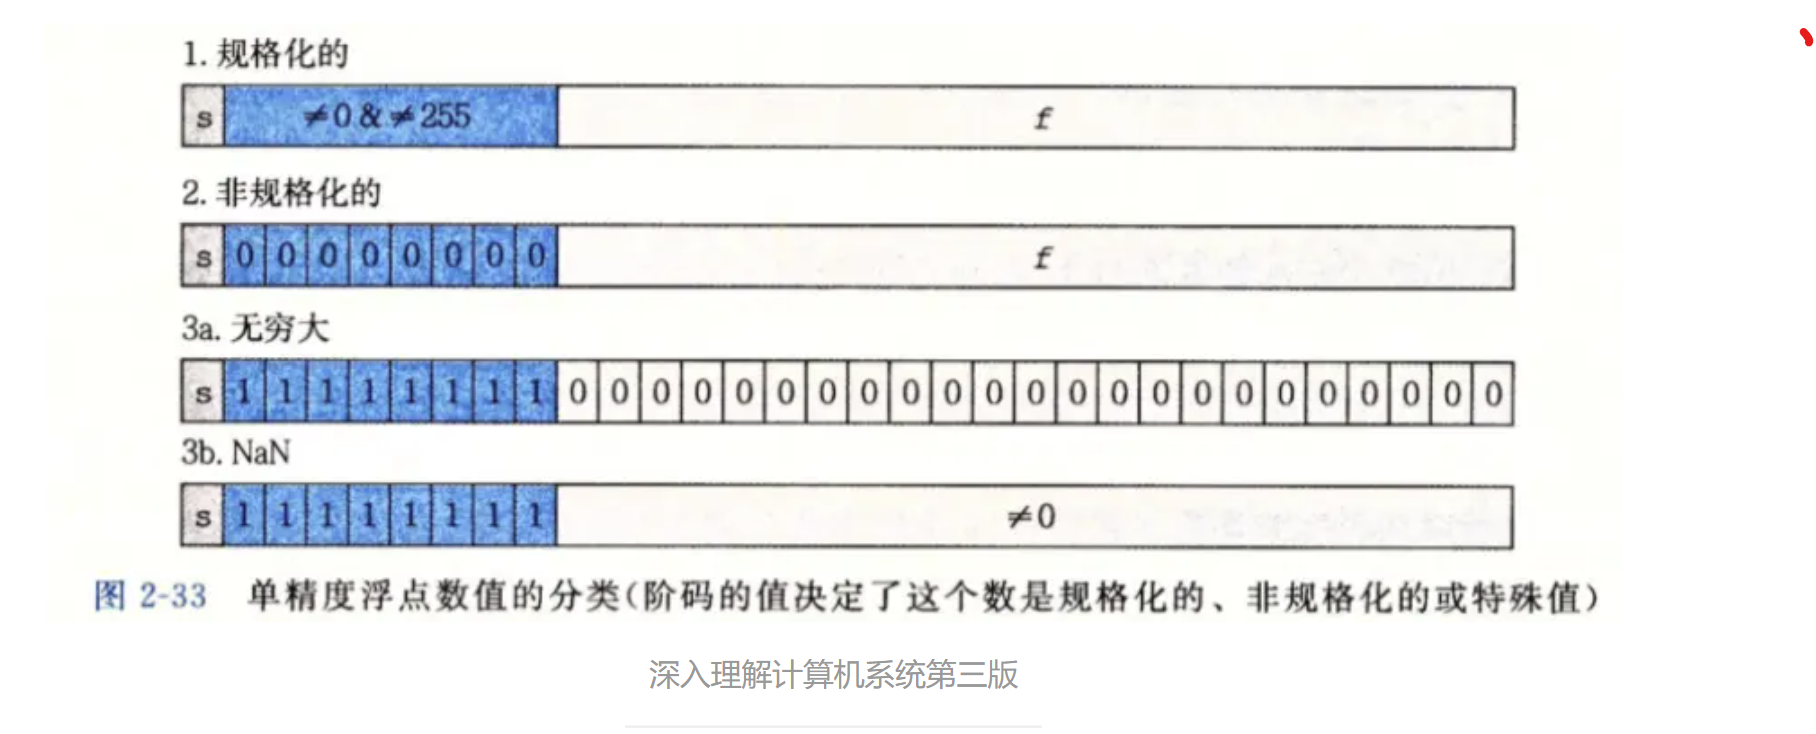
\includegraphics[scale=0.6]{IEEE754.png}
    \caption{IEEE754浮点数标准}
\end{figure}
规格化数有隐含的1,非规格化数有隐含的0
\begin{figure}[htbp]
    \centering
    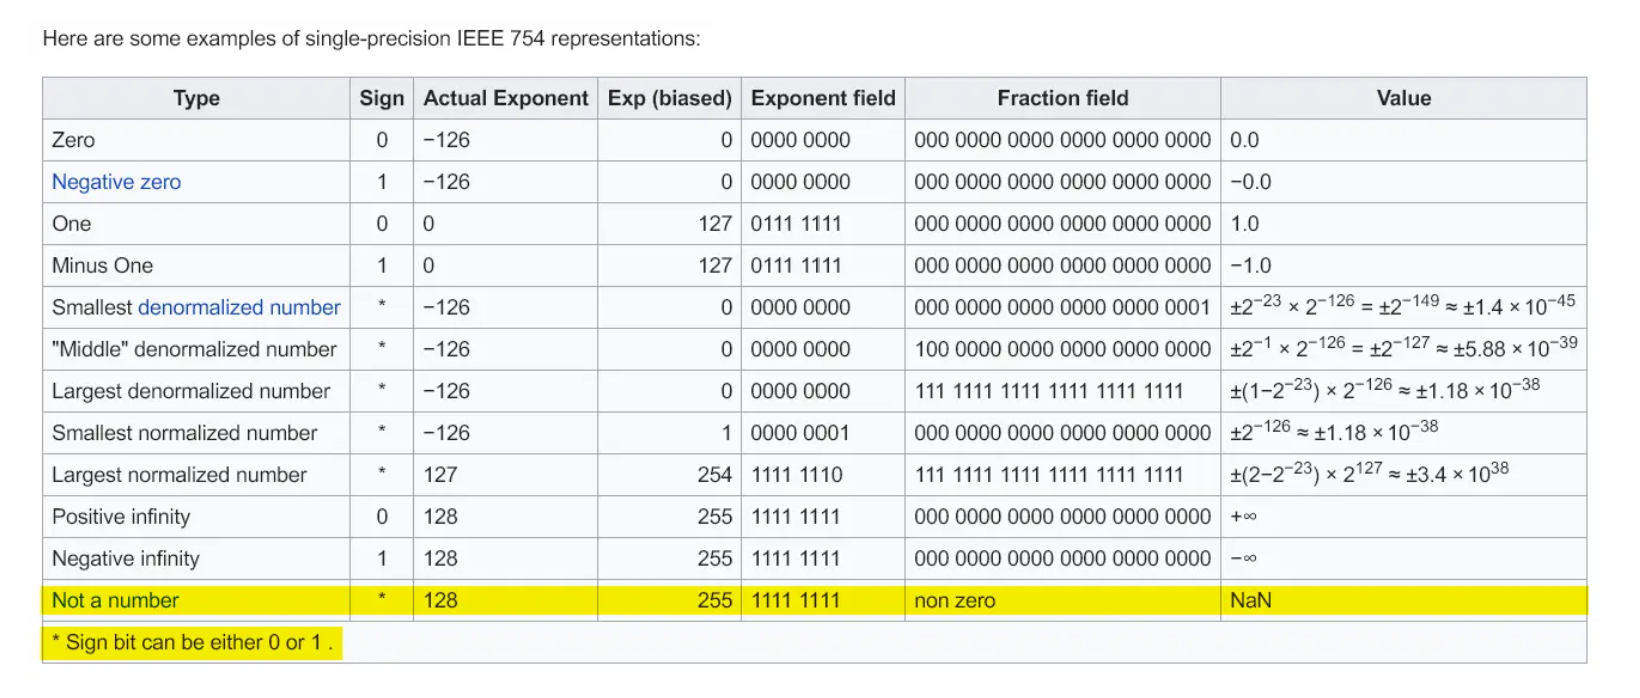
\includegraphics[scale=0.6]{IEEEnumber.png}
    \caption{特殊的IEEE浮点数}
\end{figure}

\end{document}

